\documentclass{article}
\usepackage{amsmath, amssymb, amsthm}
\usepackage{hyperref}
\usepackage{graphicx}

\title{Diffusion models and Optimal Transport}
\author{Gabriel Peyr\'e}
\date{\today}

\begin{document}

\maketitle

\begin{abstract}
	This note recaps the main ingredient of the very neat proof of Hugo Lavenant and Filippo Santambrogio~\cite{LavenantSantambrogio20} that in general, diffusion models do not define optimal transport mapping. We keep the derivation informal, the goal being to insist on the proof techniques, which is not fully constructive but relies on the nice idea of differentiating through time a family of diffusion mappings to reach a contradiction.
\end{abstract}

Generative models aim to build a transportation map $T$ between a reference distribution $\alpha$ (typically an isotropic Gaussian) and the data distribution $\beta$.
%
We denote by $T_\sharp \alpha$ the push-forward of $\alpha$ by $T$ (if $\alpha$ is made of Dirac masses at $x_i$, then $T_\sharp \alpha$ is composed of Dirac masses at $T(x_i)$). The goal is thus to find $T$ such that $T_\sharp \alpha = \beta$.
%
It is easy to see that such a map always exists for any $\beta$, but finding an explicit constructive method for $T$ is surprisingly non-trivial. Two standard approaches are optimal transport and integrating backward the advection field associated with diffusion. Two other classes of methods are flow matching (but for a Gaussian latent space, it is the same as the diffusion model up to a time reparameterization, so the same reasoning applies) and Dacorogna-Moser construction where $\beta_t = (1-t)\alpha+t \beta$ (which is problematic if the densities do not have the same support). 

\section{Optimal Transport}

Optimal transport finds $T$ by solving the Monge problem:
\begin{equation}\label{eq:monge}
    \min_T \left\{ \int \|T(x) - x\|^2 \, \mathrm{d}\alpha(x) : T_\sharp \alpha = \beta \right\}. 
\end{equation}
Brenier's celebrated theorem from 1991 states that this map exists, is unique, and can be written as the gradient of a convex function, $T = \nabla \varphi$. Conservation of mass, $T_\sharp \alpha = \beta$, equivalently means that $\varphi$ solves the Monge-Ampère equation:
\begin{equation}\label{eq:monge-ampere}
    \det(\partial^2 \varphi(x)) = \frac{\alpha(x)}{\beta(\nabla \varphi(x))}, 
\end{equation}
where the right-hand side involves the ratio of the densities of the measures. 

\section{Inverse Flow Map}

Diffusion models consider an interpolation $\beta_t$ between $\beta_0 = \beta$ and $\beta_\infty = \alpha = \mathcal{N}(0,\text{Id})$, defined by solving:
\begin{equation}
    \frac{\partial \beta_t}{\partial t} = \text{div}(y \beta_t) + \Delta \beta_t,
\end{equation}
(note that use $y$ to denote the space variable since the evolution is in the reverse direction, from the data $\beta$ to the latter variable $\alpha$) which converges to $\beta_\infty = \alpha$. The solution depends linearly on $\beta_0$ through a Gaussian convolution.

\begin{center}
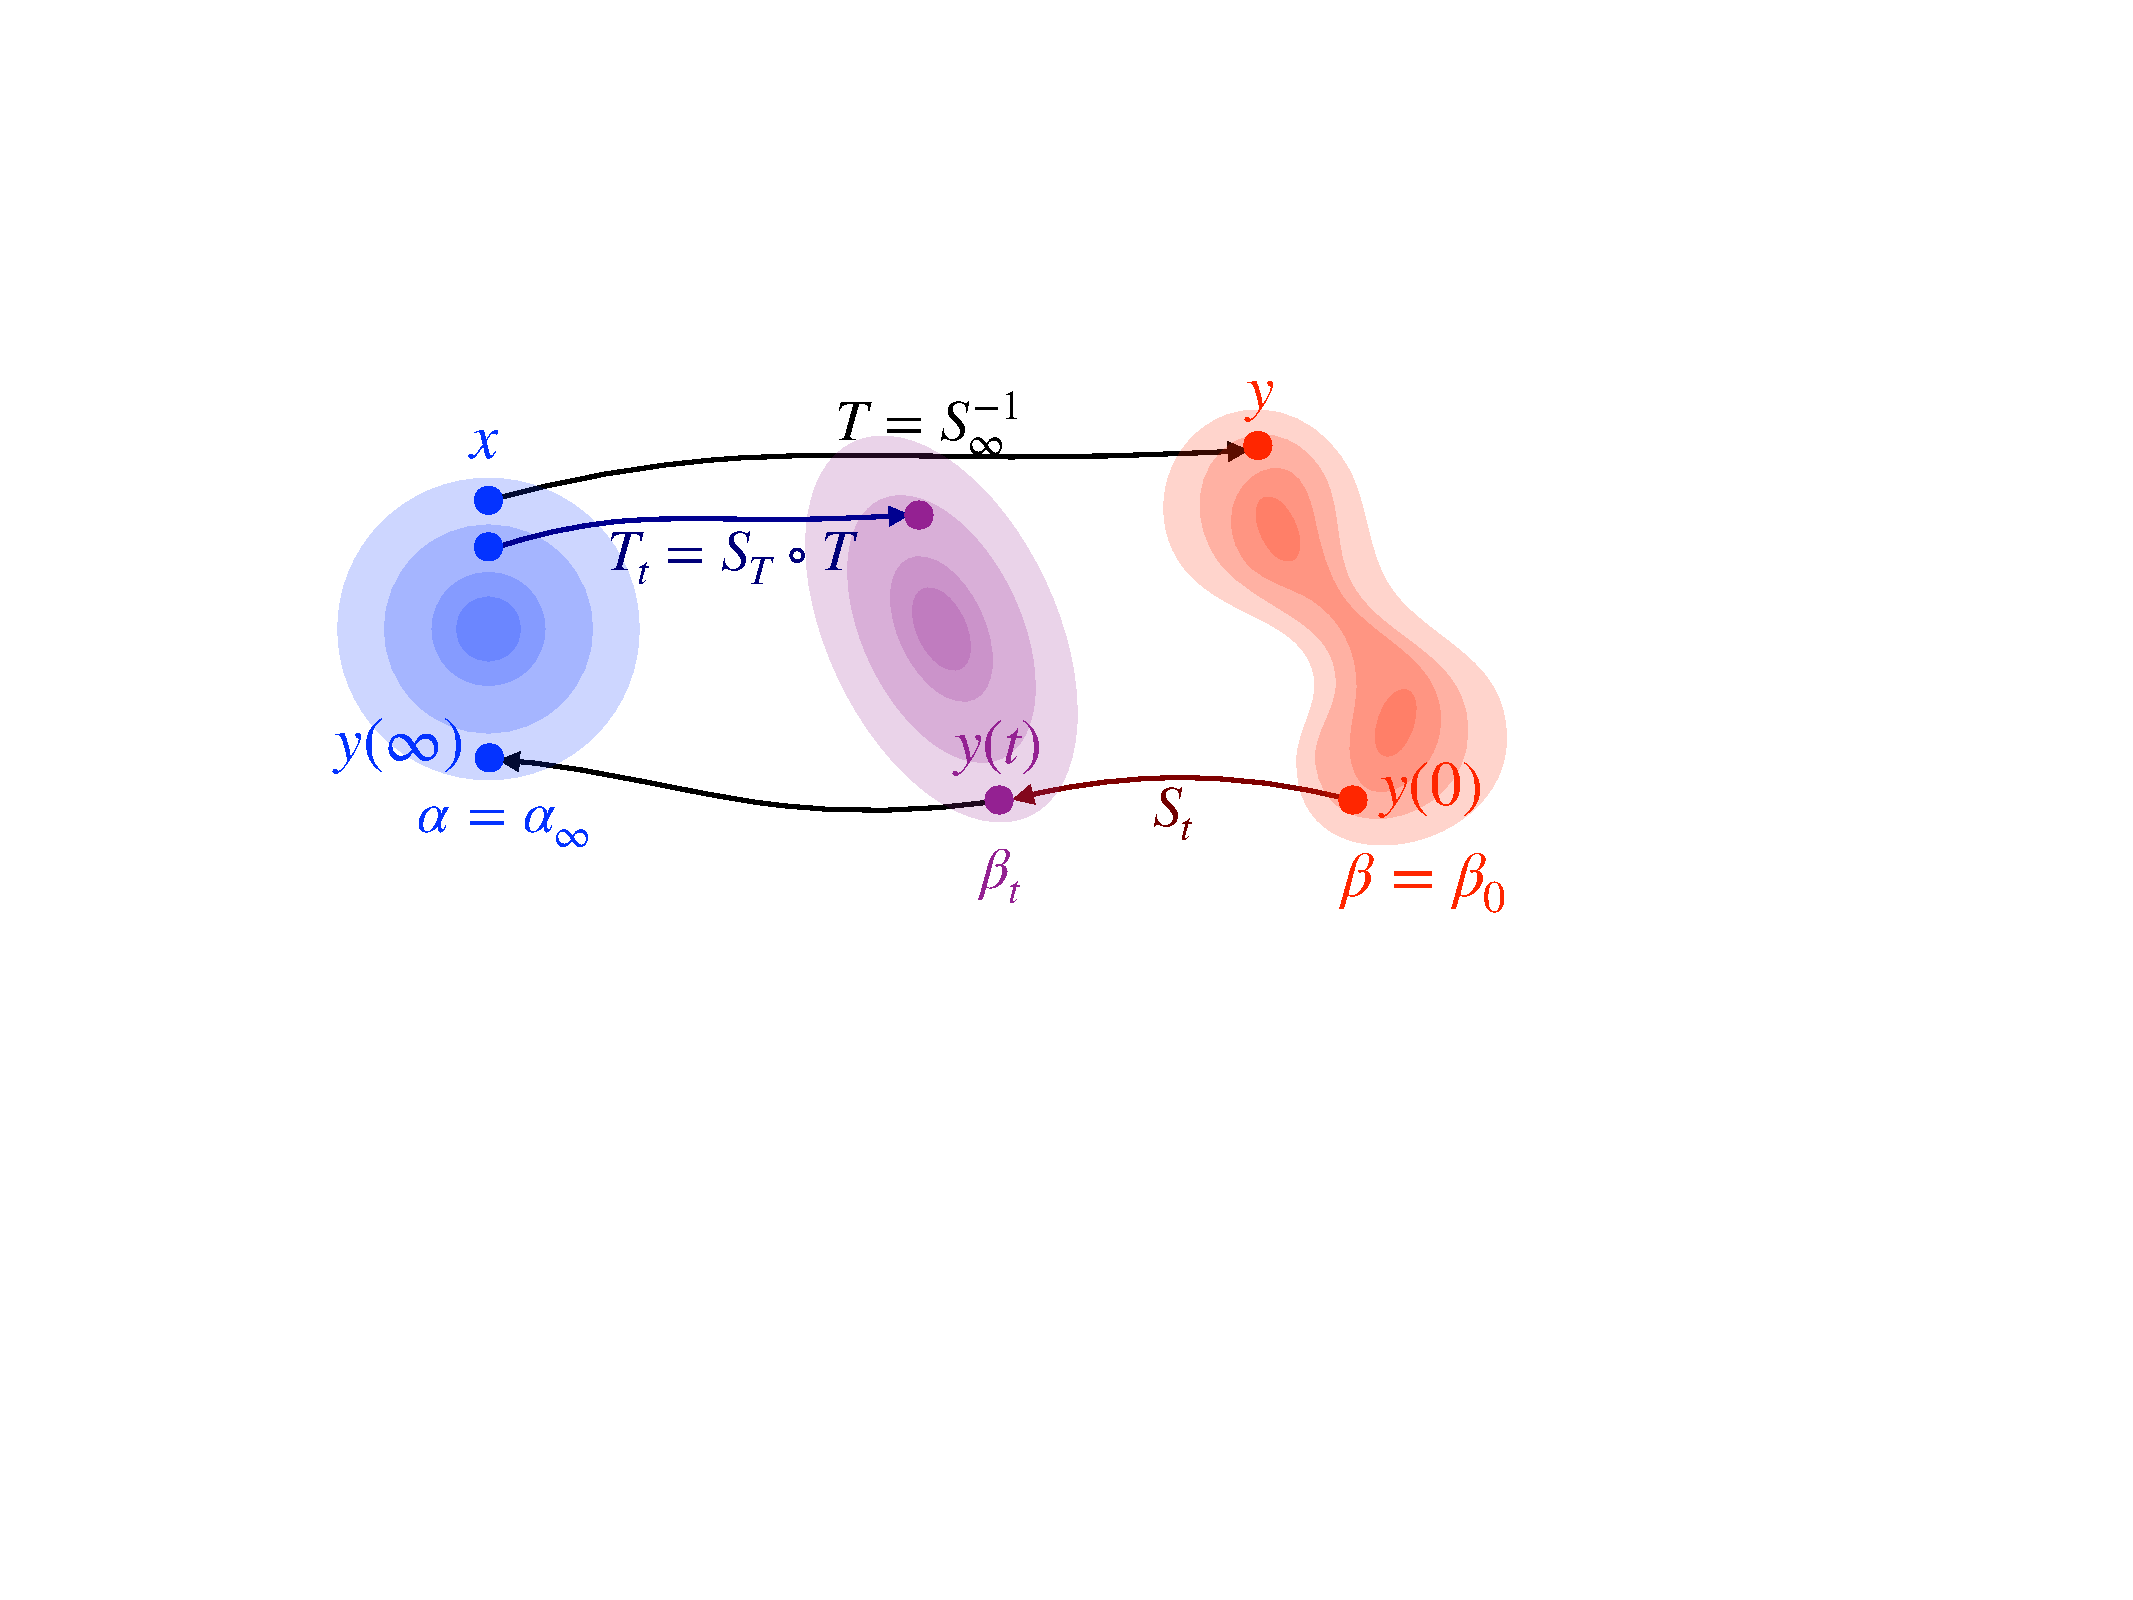
\includegraphics[width=.63\linewidth]{fig-interp.pdf}
\end{center}



Rewriting these equations in divergence form as
$$
	\frac{\partial \beta_t}{\partial t} + \text{div}[ v \beta_t ] = 0
	\quad\text{where}\quad v(y) := - y - \nabla \log(\beta_t)(y)
$$
shows that, if one has already computed $\beta_t$, then this evolution can be obtained by evolving particles according to the vector field $v$. 
%
A map $S_t$ between $\beta_0=\beta$ and $\beta_t$ is thus obtained by integrating the ODE defined by the score function $\nabla \log(\beta_t)$
\begin{equation}\label{eq:flow-ode}
    \dot{y}(t) = v(y(t)) % -x(t) - \nabla \log(\beta_t(x(t))). 
\end{equation}
The map $S_t$ is the flow map
\begin{equation}
    S_t : y(0) \mapsto y(t), \quad \text{where } y(t) \text{ solves \eqref{eq:flow-ode}} 
\end{equation}
One has $S_0 = \text{Id}$ and $(S_t)_\sharp \beta_0 = \beta_t$. Thus, in the limit $t \to \infty$, $(S_\infty)_\sharp \beta = \alpha$, so $T := S_\infty^{-1}$ is a valid transport, i.e., $T_\sharp \alpha = \beta$. We call this $T$ the \emph{inverse flow map}, which represents a deterministic diffusion model.

As a side note, the ML community is particularly excited about this idea because $\nabla \log(\beta_t)$ can be efficiently approximated from samples using denoising-based optimization. Numerically, the inverse flow map is approximated by considering a large, finite $t$ and computing $T_t = S_t^{-1}$ by integrating the ODE. In practice, a stochastic ODE is often used, making the map non-deterministic, though this requires adjusting the bias term $x$ in the ODE to account for extra diffusion.

\section{Inverse Flow Maps Are Not Optimal Transport}

It is natural to wonder whether the inverse flow map $T=S_\infty^{-1}$ is the solution to \eqref{eq:monge}. In dimension 1, $S_t$ defines a diffeomorphism, so $S_\infty$ is monotonic and so is $T=S_\infty^{-1}$. Thus, it is the gradient of a convex function, making it optimal by Brenier's theorem. If $\beta$ is Gaussian, up to a rotation of the space to make the covariance diagonal, the diffusion map is defined by a monotonic map along each axis and is also an optimal transport. A last example is the radial case, so that $\beta_t$ is also radial, and only only needs to study the radial evolution, and in this case, it is also an optimal transport.
%
The figure below shows the diffusion map for the case where $\beta$ is supported in three Dirac. In this case, the mapping defines a tesselation of the space (a Voronoi tesselation for OT) and the tesselation of diffusion is most likely different from the one of OT.   

\begin{center}
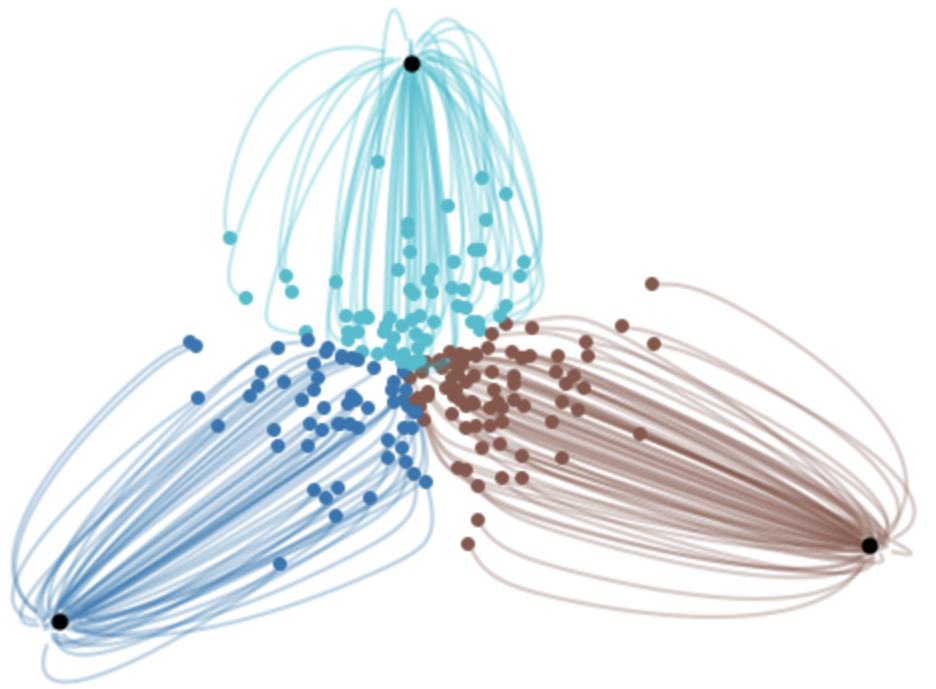
\includegraphics[width=.5\linewidth]{3-diracs.png}
\end{center}


Lavenant and Santambrogio showed by contradiction that, in general, the inverse flow map is not the optimal transport. They construct a $\beta$ close to the isotropic Gaussian $\alpha$, but instead of proving the conjecture is false for $\beta$, they show there exists some $t \geq 0$ such that the inverse flow map $T_t$ from $\alpha$ to $\beta_t$ is not an optimal transport. They actually shows that $T_t$ is not an optimal transform for $t$ which can be arbitrary close to 0 (but not necessarily 0 \ldots).

We denote $S_t$ the flow map from $\beta_0 = \beta$ to $\beta_t$. If the conjecture is true, the inverse flow map $T_t$ from $\alpha$ to $\beta_t$ is an optimal transport for all $t$. By the composition rule of flow maps, this map is:
\begin{equation}
    T_t := S_t \circ S_\infty^{-1} = S_t \circ T,
\end{equation}
and $(T_t)_\sharp \alpha = \beta_t$. The goal is to show that $T_t$ being an optimal transport for all $t$ leads to a contradiction if $\beta$ is well-chosen (specifically, very close to $\alpha$ with specific second- and fourth-order log-density derivatives at 0).

By Brenier's theorem, $T_t$ being an optimal transport implies that it is the gradient of a convex function, which is equivalent to:
\begin{equation}\label{eq:sym}
    \partial T_t(x) \text{ is a positive symmetric matrix for all } x \text{ and } t. 
\end{equation}
Combining:
\begin{itemize}
\item Differentiating \eqref{eq:sym} with respect to $t$,
\item Differentiating the flow ODE \eqref{eq:flow-ode} with respect to $x$,
\end{itemize}
and then evaluating the obtained equation at $t = 0$, Hugo and Filippo showed by explicit computation that this leads to:
\begin{equation}\label{eq:interm-eq}
    [\partial^2 \log(\beta)(T(x))] \times [\partial T(x)] \text{ is symmetric.} 
\end{equation}

Using the fundamental property:
\[
    A, B \text{ symmetric and } AB \text{ symmetric } \iff AB = BA,
\]
it follows that \eqref{eq:interm-eq} implies:
\begin{equation}
    \forall y = T(x), \quad G(y) := \partial^2 \log(\beta)(y) \text{ commutes with } H(y) := \partial S_\infty(y).
\end{equation}

To reach a contradiction, assume $G(y)$ and $H(y)$ commute for all $y$. Since $\beta = T_\sharp \alpha$, $\alpha = S_\sharp \beta$, and $T$ and $S$ are inverse optimal transport maps, we denote $S = \nabla \psi$ with $\psi$ convex. The Monge-Ampère equation \eqref{eq:monge-ampere} implies:
\begin{align*}
    G(y) &= \partial^2 \log(\beta)(y) = \partial^2 \left[\log\det(\partial^2 \psi) - \frac{1}{2} \|\nabla \psi\|^2\right](y), \\
    H(y) &= \partial S_\infty(y) = \partial^2 \psi(y).
\end{align*}

To make $\beta$ close to $\alpha$, consider:
\[
    \psi(y) = \frac{\|y\|^2}{2} + \varepsilon h(y),
\]
for small $\varepsilon$. Expanding in Taylor series, after some computation:
\begin{align*}
    G(y) &= -\text{Id} + \varepsilon \{\partial^2[\Delta h] + \partial^2[y \cdot \Delta h]\} + o(\varepsilon), \\
    H(y) &= \text{Id} + \varepsilon \partial^2 h(y).
\end{align*}

Focusing on $y = 0$, the goal is to reach a contradiction by crafting $h$ such that  $\partial^2 h(0)$  and   $\partial^2[\Delta h](0)$ do not commute. 
 %
Around $0$, $h$ must be at least a polynomial of degree 4. An example in dimension 2 is:
\[
    h(y) = y_1 y_2 + y_1^4,
\]
yielding:
\[
    \partial^2 h(0) = \begin{pmatrix} 0 & 1 \\ 1 & 0 \end{pmatrix}, \quad 
    \partial^2[\Delta h](0) \propto \begin{pmatrix} 1 & 0 \\ 0 & 0 \end{pmatrix}.
\]

\begin{thebibliography}{9}
    \bibitem{LavenantSantambrogio20}
    H. Lavenant and F. Santambrogio, \emph{The flow map of the Fokker--Planck equation does not provide optimal transport}, SIAM Journal on Mathematical Analysis, 2020.
\end{thebibliography}

\end{document}